\documentclass[runningheads,a4paper]{llncs}

\usepackage{amssymb}
\setcounter{tocdepth}{3}
% for figures
\usepackage{graphicx}
\usepackage{tikz}
% for tables
\usepackage{longtable}
\usepackage{booktabs}
\usepackage{rotating}
% for listings
\usepackage{listings}
\usepackage{url}
\urldef{\mailsa}\path|marcelo.hidalgo@hcu-hamburg.de|
\newcommand{\keywords}[1]{\par\addvspace\baselineskip
\noindent\keywordname\enspace\ignorespaces#1}
\begin{document}
\lstset{language=R} 
\mainmatter% start of an individual contribution

% first the title is needed
\title{A National Heat Demand Model for Germany}

% a short form should be given in case it is too long for the running head
\titlerunning{A National heat Demand Model for Germany}

\author{Marcelo Esteban Mu\~noz Hidalgo}
\authorrunning{A National heat Demand Model for Germany}

\institute{
%\textbf{Prepared for:
%1st Workshop on Agent Based Modelling of Urban Systems (ABMUS 2016)\\
%\url{http://www.modelling-urban-systems.com/}}\\
%\vspace{0.5cm}
HafenCity Univerity, Urban Planing\\
\"Uberseealle 16, 20457 Hamburg, Germany\\
\mailsa}

\toctitle{A National Heat Demand Model for Germany}
\tocauthor{M. Esteban Mu\~noz H.}
\maketitle

\begin{abstract}

Spatial microsimulation models can be used for the analysis of complex systems.
In this paper we make use of a spatial microsimulation model for the
estimation of heat demand for Germany at a NUTS--3 level.
The presented model creates a synthetic building stock by re-weighting the
national microdata sample to small areas (NUTS--3) statistics with help of the
GREGWT algorithm.
Using the GREGWT method we benchmark the microdata sample to three different
aggregation units (a) the building level (i.e.\ number of buildings); (b)
families/dwelling units; and (c) individuals.
\\

The model takes into account the different climate regions defined on the
national German 18599-DIN standard.
In order to incorporate the climate data into the model, we make use of a quasi
steady-state heat transfer model to compute the heat demand of the individual
buildings.
These type of models require a building geometry for the estimation of heat
demand, in this case we do not have information of the individual building
geometry but only about the building size, expressed as square meters.
We define synthetic geometrical boxes for the computation of heat demand.
\\

The described model is able to represent the national building stock at a
microlevel.
These type of models are essential for the assessment of policies targeting
(a) the reduction of carbon emissions in the construction sector and
(b) the increase of energy efficiency on heat distribution grids.
\\

\keywords{GREGWT, Heat Demand, Synthetic Building Stock, Spatial Microsimulation}
\end{abstract}

\section{Introduction: The Need of a National Energy Demand Models at a Microlevel}

Energy supply systems of most developed countries are facing a rapid
transition towards carbon neutral infrastructures.
Part of this transition has proven to be a decentralization of energy supply sources.
This decentralization of supply has introduced many new actors into the system.
This decentralization is not only a spatial decentralization but a
decentralization of energy production capacities.
We see a trend towards the supply of urban and rural areas through distributed
systems with a much lower energy production capacity.
In order to understand this type of systems we need to develop models able to:
(a) describe the distributed systems at their output aggregation level;
(b) capture the diversity of the individual systems; and
(c) integrate national policies influencing the development of these systems
and the population affected by these policies.
\\

The use of a spatial microsimulation model for the description of these complex
systems is ideal.
With a spatial microsimulation model we are able to generate a synthetic
building stock benchmarked to small areas (NUTS--3 level).
An internal validation of the model shows that it is performing with high
accuracy (see Section~\ref{subsec:performance}).
The synthetic building stock is enriched with energy relevant parameters--
mainly heat transmission coefficients-- needed for the computation of heat
demand.
With this enriched building stock we can perform many types of simulations.
In this paper we simulate the monthly heat demand of the synthetic building
stock.
The spatial microsimulation model allows us to represent the entire building
stock of Germany at a micro level with a monthly resolution.
The simulation of heat demand at a higher temporal resolution can be achieved
through the use of a thermal simulation model instead of the implemented
quasi steady-state heat demand model.
\\

An innovation of this model is the consideration of climate zones for the
estimation of heat demand.
We classify the individual small areas into predefined climate zones.
A climate zone is defined by the monthly mean outside temperature and by its
monthly solar radiation.
Both variables are given as input to the heat demand model.
\\

We structured the paper into five main sections:
on Section~\ref{sec:heat} we make a brief description of the implemented heat
demand model and the used input parameters, on this section we also describe
the enrichment process of the microdata sample with energy relevant parameters;
on Section~\ref{sec:climate} we describe the defined climate zones;
on Section~\ref{sec:microsim} we describe the implemented algorithm and
procedure for the re-weighting of the enriched microdata;
on Section~\ref{sec:result} we present and discuss the main results from the
performed simulation;
we conclude the paper with Section~\ref{sec:conclusions} where we draw our
conclusions from the simulation results and present an overview of the steps
ahead as well as other possible implantations of the developed model.
\\

\section{The Heat Demand Model}\label{sec:heat}

The computation of heat demand occurs at a micro level.
We construct a synthetic building for each individual in the microdata sample,
the resulting heat demand is divided by household-size.
This means that we need to define a building geometry for each individual in
the census.
We use the average dwelling unit size from the microdata sample for the
definition of number of stories of single family houses.
E.g\ if an individual from the microdata sample lives on a single family house
with a floor space of 120~$m^2$ and the computed average dwelling unit size
from the sample is 60~$m^2$, we define the geometry of the building as a two
storey building, each storey with a floor space of 60~$m^2$.
Multi-family houses are simulated as single storey buildings, e.g.\ each
dwelling unit of the multi-family house is simulated as a one storey building.
\\

Each individual on the microdata sample describes the building they live in with
three characteristics: (1) dwelling unit size, in square meters; (2)
construction year of the building; and (3) number of dwelling units on the
building. With these three parameters we classify the microdata sample into building
typologies. We make use of a well established building typology in Germany, the
IWU typology~\cite{Diefenbach.2010b,Loga.2011}. This process allows us to
enrich the microdata sample with energy relevant parameters. Out of the
predefined typologies we take important parameters needed for the estimation of
heat demand. Probably the most important parameters we take out of the building
typology are heat transmission coefficients of building parts (roof, ceiling,
walls and windows), we also define the percentage of glazing area of the
buildings based on this typology.
All these parameters are given as input variables to the quasi steady-state heat
demand model.
\\

The use of building typologies for the construction of either: (a) urban heat
demand models working at a microlevel, e.g.\ by classifying the digital
cadastre into building types; or (b) aggregated national models can be found
throughout the
literature~\cite{Caputo.2013,Hrabovszky.2013,Kragh.2013,Singh.2013,DallO.2012,Dascalaki.2011,Balaras.2007}.
This paper presents a method that combines these two approaches: a model working at
a microlevel able to asses the impact of national policies relevant to the
energy efficiency of the building stock.
\\

The IWU typology defines each building type by construction epoch and building
type. Table~\ref{tab:IWU-de} lists the predefined typologies with the defined
heat demand value of the building type. In our model we do not use this value
but the underlying parameters used for the computation of the presented heat
demand value of each building type.
We need to make use of the underlying parameters, rather than the heat demand
values in order to: (1) compute the heat demand at a higher temporal
resolution; and (2) open the door for a projection of the building stock under
different policies targeting the retrofitting of existing buildings.
\\

\begin{table}[htbp]
  \centering
  \caption{IWU-de building typology matrix for Germany}\label{tab:IWU-de}%
    \begin{tabular}{l r rrr rrr rrr r}
    \addlinespace
    \toprule
    &
    \begin{sideways}\textless~1859\end{sideways}&  %01
    \begin{sideways}1860--1918\end{sideways}&     %02
    \begin{sideways}1919--1948\end{sideways}&     %03
    \begin{sideways}1949--1957\end{sideways}&     %04  
    \begin{sideways}1958--1968\end{sideways}&     %05  
    \begin{sideways}1969--1978\end{sideways}&     %06  
    \begin{sideways}1979--1983\end{sideways}&     %07  
    \begin{sideways}1984--1994\end{sideways}&     %08  
    \begin{sideways}1995--2001\end{sideways}&     %09  
    \begin{sideways}2002--2009\end{sideways}\\    %10
    \midrule
EFH$^a$&183&180&164&181&146&155&118&132&110&88\\
RH     &   &153&137&156&106&127&127& 98& 78&86\\
KMH    &190&143&168&156&129&134&118&122& 92&79\\
GMH    &   &127&144&142&131&117&   &   &   &  \\
HH     &   &   &   &   &114&113&   &   &   &  \\
    \bottomrule
    \addlinespace
    \end{tabular}\\
    \begin{footnotesize}    
    source:~\cite{Loga.2011} 
    Specific Heat demand (spez. W\"armebedarfskennzahl)
    $[kWh/m^{2}a]$\\
(EFH) Single family house ``Einfamilienhaus'';
(RH) Terrace house ``Reihenhaus'';
(KMH) Apartment house ``Mehrfamilienhaus'';
(GMH) Large apartment house ``Großes Mehrfamilienhaus'';
(HH) High-rise ``Hochhaus'';
    \end{footnotesize}
\end{table}


The computation of heat demand is performed with a quasi steady-state model
implemented in the R language~\cite{MunozH.2015.heat}. This is an
implementation of the German norm DIN~18599~\cite{DIN.18599.V}.
This norm is used for the heat demand computation of energy performance
certificates of new and existing buildings in Germany.
\\

The computation of heat demand is a balancing procedure between \textit{heat gains}
$Qg$ and \textit{heat losses} $Ql$. The difference between them is the needed
heat demand to maintain a predefined internal temperature set-point of the dwelling unit.
The internal temperature set-point in this model is fixed, we use the defined internal
temperature of the DIN norm. Because we use the microdata sample for the estimation of
heat demand, we have a rich description not only of the building stock but also
about their residents, this data can be used for the definition of user
parameters like internal temperature set-point,
see~\cite{MunozH.2014.IBPSA-JP,MunozH.2015.IBPSA.Pop} for this type of
implementations.
\\

The monthly heat demand $Qh$ is computed using the estimated monthly heat gains
$Qg$ and monthly heat losses $Ql$, see Equation~\ref{eq:Qh}, where $m$ is the
month of the year.
The heat demand is defined as the needed heat to maintain the operative
temperature and cover the heat losses.
A fraction of all the computed heat gains are subtracted from the heat losses, 
this fraction is the usable share of the total heat gains. 
The fraction is computed with help of the \textit{eta} ($\eta$) Factor.\\

\begin{equation}\label{eq:Qh}
    Qh = Ql - \eta \times Qg
\end{equation}
\\

The monthly heat gains $Qg$ are computed as the average monthly solar heat flow
$Ss$ plus the heat flow by internal heat sources $Si$, both measured in $[W]$,
see Equation~\ref{eq:Qg}. The monthly solar heat flow is computed based on:
(a) the monthly solar radiation, defined by the climate zone; (b) the share of
glazing surface, defined by the building typology; and (c) the building
orientation, neglected on this model. The internal heat sources are fixed on
this implementation. Similar to the internal temperature set point, this
variable can be modeled as occupant behaviour.
\\

\begin{equation}\label{eq:Qg}
    Qg = 0.024 \times (Ss + Si) \times t
\end{equation}
\\

The computed heat losses $Ql$ are computed as the specific total heat loss
$H$ measured in $[W/K]$ times the difference between the inside temperature
(or temperature set point) $Ti$ and the outside ambient temperature $Te$,
measured in kelvin $[K]$, see Equation~\ref{eq:Ql}. The internal temperature is
set fix throughout the model while the monthly outside temperature varies
between climate zones.
\\

\begin{equation}\label{eq:Ql}
    Ql = 0.024 \times H \times \left(Ti-Te\right) \times t
\end{equation}
\\

The most important factors of the specific total heat loss in our model are the
transmission losses $Ht$. The transmission losses are computed as the sum of
transmission losses of all building components encountered with ambient air.
The individual transmission losses are computed as the heat transmission
coefficient $U$ of the building component (normally referred as the U-value, or
R-value) measured in $[W/(m^2K)]$ times the corresponding building component
surface area $A$, measured in $[m^2]$. The heat transmission coefficients of
the individual building components are defined through the building typology.
The area of the components is taken out of the generated building geometry. The
generated geometry is computed as function of the dwelling unit size. 
Equation~\ref{eq:Ht} depicts this computation step. Other heat losses are
thermal bridges and ventilation losses. In our model the ventilation losses
are fixed throughout the model. This variable, analog to internal temperature
set-point and internal gains, could be modeled as occupant behaviour.
\\

\begin{equation}\label{eq:Ht}
    Ht = \sum_{i=1}^{n} \left(U_{(i)} \times A_{(i)}\right)
\end{equation}
\\

An example of this computation is depicted on Figure~\ref{fig:heat} for a
random building for all predefined climate zones. An example of the used code
for the computation of heat demand for the example shown on Figure~\ref{fig:heat} is
listed below.\\

\begin{lstlisting}
library(heat)
result <- heat(output_type='Month', climate='Hamburg')
\end{lstlisting}
\\\vspace{0.5cm}

This method is normally used at a monthly resolution but can be used to
simulate heat demand in a more granular temporal resolution. For now we limit the
simulation to a monthly resolution because of the available climate data for
the predefined climate regions in Germany, see next section for a description of
this data.
\\

\begin{figure}
\centering
\includegraphics[width=0.7\textwidth]{FIGURES/heat.png}
\caption{Computed monthly heat demand for all climate zones}\label{fig:heat}
\end{figure}

\section{Defined Climate Regions in Germany}\label{sec:climate}

The simulation of heat demand for the entire country requires an explicit
consideration of regional climatic conditions.
In this paper we present the use of climate zones for the consideration of
climate variation of different regions in Germany.
Figure~\ref{fig:climateZones} shows the 15 predefined climate zones
in Germany.
These climate zones are defined in the German DIN norm
DIN~18599~\cite{DIN.18599.V}.
The norm also provides the necessary climate-data for a monthly estimation of
heat demand.
For the computation of heat demand at a different temporal resolution
implementing a quasi steady-state model we would require climate data with the
same temporal resolution.
\\

\begin{figure}
\centering
\begin{tabular}{lr}
\includegraphics[width=0.6\textwidth]{FIGURES/climateZones.png}&
\includegraphics[width=0.3\textwidth]{FIGURES/climateZones_legend.png}
\end{tabular}
\caption{Defined climate regions for the computation of heat
demand}\label{fig:climateZones}
\end{figure}

We modify the implemented quasi steady-state model used in this paper in order
for it to be aware of the climate regions, making it possible for us to define the
desired region simply by name. The implemented R library loads all the climate data on
startup and selects the needed data for the estimation of heat demand based on
the user input.
\\

%For the re-weighting of the microdata sample we use a sub-sample of it based on
%the federal state of the simulation areas (see Section~\ref{sec:microsim}),
%federal states are plotted in red on Figure~\ref{fig:climateZones}.
%This presents a conflict because, the federal states and the climate zones do
%not perfectly overlap. Because of this overlapping we had to create a unique
%sub-sample of the microdata sample for each climate region composed of the
%federal states that the climate zone overlaps with.
%\\
%
%For each individual of each sub-sample of the microdata sample we compute their
%heat demand.
%Each sub-sample takes different climate data as input for the computation of
%heat demand.
%We perform this computation for each individual a certain number of times
%depending on the sub sampling of the microdata sample.
%Because of the overlapping between climate zones and federal states, the same
%record on the microdata sample can be used more than one time within the
%simulation.
%\\

We compute the heat demand of each individual on the survey sample previous to
the re-weighting of the sample, see Section~\ref{sec:microsim} for the
re-weighting procedure.
In order to incorporate the climate data, define by the climate zones, we could
compute the monthly heat demand of each individual for each predefined climate
zone.
After the re-weighting procedure we would just have to select to climate zone
corresponding to the NUTS--3 geographical area.
This procedure is not very efficient.
For the re-weighting procedure we do not use the entire sample survey, but
select the records corresponding to the federal state (NUTS--1 level).
This means that only climate zones overlapping a given federal states are
relevant for all NUTS--3 geographical areas within that federal state.
With this in mind we can define which climate zones to use for the computation
of heat demand of each individual in the sample survey.
A small example.
The federal state of North Rhine-Westphalia (see Cologne on
Figure~\ref{fig:climateZones}) overlaps with two climate zones:
(5) Essen; and (6) Bad Marienberg.
The re-weighting process for all NUTS--3 areas within this state will either
select climate zone 5 or 6, but never use climate zone 7.
For that reason, for individuals within the NUTS--1 region of North
Rhine-Westphalia,
we only need to compute the heat demand twice (with climate data from zone 5
and 6) instead of 15 times (for each climate zone).
\\

The implementation of climate data at a higher spatial resolution at the same
temporal resolution is possible. There is available climate data at a very
small spatial resolution. It might be even possible to define climate
data at a small area level. There are two major concerns with such an approach:
(1) the number of computations of heat demand would exponentially increase,
we would need to compute the heat demand of each individual of the microdata
for each small area rather than for each sub sample,
running such a computational intensive model could shut the doors to more
interesting modeling techniques like the projection of the building stock into
the future; and (2) energy efficiency policies are attached to estimations
based on the data provided by the German DIN norm.
In this case a higher fidelity of the model does not mean a better
representation of reality.
\\

\section{The Spatial Microsimulation Model}\label{sec:microsim}

Microsimulation, introduced by~\cite{Orcutt.1957}, is a commonly used method
among many social scientist. This method has been used to simulate a large
range of social phenomena at a micro-level. The first step of this method is
normally the generation of a synthetic population representing the population
under analysis. The spatial microsimulation methodology extends this concept by
allocating estimated synthetic populations to geographical
areas~\cite{Clarke.1987}. For overview of spatial microsimulation models, its
applications and methods see~\cite{Tanton.2014,ODonoghue.2014}. For the
presented model we use the 
\textbf{G}eneralised \textbf{REG}ression and \textbf{W}eigh\texbf{T}ing of
sample survey results, knows by its acronym GREGWT.
We use the available GREGWT R library~\cite{MunozH.2015.GREGWTR}, this library
is an implementation of the GREGWT algorithm. The GREGWT algorithm was
originally developed by the Australian Bureau of Statistics
(ABS)~\cite{Bell.2000}. This algorithm is used by the National Center for
Social and Economic Modeling (NATSEM) on their spatial microsimulation model
spatialMSM~\cite{Tanton.2007,Tanton.2014a}.
\\

The simulation process computes the weights for each area iteratively.
Although the R simulation library GREGWT can internalize this process, we need to
run the loop outside the library environment in order to store the data on disk
efficiently. This type of simulation generates almost 8Gb of data, this can be
a problem if we try to store a large R data frame on RAM. The code below is a
simplified representation of the simulation process.
\\

\begin{lstlisting}
library('GREGWT')
for (area in small_areas){
    weights = GREGWT(simulation_data, area_code=area)
}
\end{lstlisting}
\\

The lowest possible geographical identification on the microdata survey is the
federal state (NUTS--1). For the re-weighting process at the small areas we only use the
records of the corresponding federal state (e.g\ if a small area is within
the federal state of Bavaria, we will only re-weight records from the microdata
survey identified to the federal state of Bavaria).
%In order to accelerate the
%computational process we do not compute heat demand for each climate zone for
%each individual on the microdata survey. Because we only use a sub sample of
%the microdata survey depending on the federal state for the re-weighting
%process, we only need to compute the heat demand of each individual for the
%climate zones within the corresponding federal state.
\\

For each simulation area we compute a new set of weights, this weights are
stored on csv files. We use these weights to compute the total heat demand of
each simulation area. The heat density is computed as the total heat demand
divided by the area size expressed as $[Wh/ha*month]$.
\\

\subsection{Data}

In order to define the synthetic building stock we re-weight the 2010 German
microdata survey~\cite{NRW.2010}. The re-weighting process is benchmarked to
aggregated statistics from the 2011 German census~\cite{NRW.2011} available at
a NUTS-3 level. The used benchmarks are listed on Table~\ref{tab:data}.
\\

\begin{table}[htb]
    \centering
    \caption{Used benchmarks from the 2011 Census and corresponding micro
    census attributes}\label{tab:data}
    \begin{tabular}{lllp{5.5cm}}
        \toprule
        \textbf{MC Code$^*$}\cite{NRW.2010} &
        \textbf{Census Code}\cite{NRW.2011} &
        \textbf{Unit$^{**}$} &
        \textbf{Description}\\
        \midrule
EF1       & / & /      & Federal State (NUTS--1)\\
EF952     & / & Person & Weight\\
EF44      & ALTER\_KURZ      & Person    & Age (five classes of years)\\
EF49      & FAMSTND\_AUSF    & Person    & Marital status (in detail)\\
EF46      & GESCHLECHT       & Person    & Sex\\
EF20      & HHGROESS\_KLASS  & Person    & Size of private household\\
          \midrule
EF492     & WOHNFLAECHE\_20S & Dwelling  & Floor area of the dwelling (20$m^2$ intervals)\\
          \midrule
EF494     & BAUJAHR\_MZ      & Building  & Year of construction (microcensus classes)\\
EF635     & ZAHLWOHNGN\_HHG  & Building  & Number of dwellings in a building\\
\bottomrule
\multicolumn{4}{l}{$^*$Micro Census Code}\\
\multicolumn{4}{l}{$^{**}$Refers only to Census}
    \end{tabular}
\end{table}


% tab:data

The census data is directly retrieved from the census webpage for each
benchmark iteratively. The combined census data contains 11300 NUTZS-3 areas and
7 benchmarks described with a total of 44 categories. The microdata sample contains
a total of 528 attributes and 489330 records. Out of the 528 attributes we only
use the 7 attributes corresponding to the census benchmarks plus the original
survey design weights and the federal state geographical identification number.
\\

\subsection{GREGWT}

GREGWT is an implementation of method number 5
of~Sigh~\&~Mohl~\cite{SinghMohl.1996}. Tanton~\cite{Tanton.2011a} makes a
detailed description of the algorithm and its applications. The mathematical
description of the GREGWT algorithm presented below is taken
from~\cite{Rahman.2010} and the algorithm description
from~\cite{MunozH.2015.IMA.GREGWT}.
\\

Aim of the GREGWT algorithm is to find a set of new weights $w$ that can be
used to match the microdata survey $X$ to a set of given benchmarks $T$ (in
this case NUTS--3 small area statistics) so that $T = \sum w_{j} X_{j}$ while
minimizing the weight difference between the new weights $w$ and the sample
design weights $d$ from the microdata survey.
%
Note that $T$ is given at a higher resolution (aggregated to the predefined
geographical areas, NUTS--3 in this case) than the microdata sample.
Thus, the re-weighting procedure computes a new set of weights for 
the microdata records so that the properties of $T$ are generated, with the
additional property that the new weights should be
close to the old weights.
%
For the distance $D$ between design and estimated weights the GREGWT algorithm
makes use of the truncated Chi-Squared distance function, represented in
Equation~\ref{eq:distance}.
\\

\begin{equation} \label{eq:distance}
    D = \frac{1}{2} \sum_j \frac{{\left(w_j - d_j \right)}^2}{d_j}
\end{equation}
\\

%The distance minimization equation is expressed as the Lagrangian function of
%the Chi-Squared function. With this equation we can formulate an equation for
%the new weights. Where $X^{'}_j = \sum \lambda_k X_{j,k}$.
%\\
%
%\begin{equation}
%    w_j = d_j + d_j X^{'}_j
%\end{equation}
%\\

This is a constrained optimization problem where $D$ is minimized subject to
the constraints $T = \sum w_j X_j$.
\\

Now given the new survey weights $w_j$ for a NUTS--3 geographical area $i$, we
compute the overall heat demand $H$ of the geographical area as:
\\

\begin{equation}
    H_i = \sum_i \sum_j w_{i,j} * Qh_{i,j}
\end{equation}

Where $Qh_{i,j}$ is the computed heat demand for individual $i$ of the sample
microdata and climate zone of geographical area $j$.
$Qh$ is given by Equation~\ref{eq:Qh}.
\\

For a spatial microsimulation model we need a last step. The algorithm needs a
weight restriction in order to avoid negative weights, in such case the algorithm
implements an iterative process to maintain a low weight distance within the
weight constraints. The R GREGWT implementation defines boundaries constraints as
a user input. The user can define an upper and lower bound. If the algorithm
computes weights outside these bounds, the weights will be truncated to the
predefined bounds. In this case the algorithm will iterate with the new computed
weights until a predefined convergence parameter is met or there is no
improvement in the iteration.
\\

\subsection{Benchmarking to Different Aggregation Units}\label{sec:bench}

The used census benchmarks of the small areas count different aggregation
units: (1) Individuals/People, (2) Families/Dwelling units, and (3) Buildings
(see Table~\ref{tab:data}). Our R library used for the re-weighting of survey
data is able to perform an integrated re-weight. This can be useful for a
re-weighting of the microdata survey for which maintaining the original family
structure of the data set is important. An integrated re-weight does not give us the
possibility to benchmark the survey to more than two aggregation units.
%
The aim of this paper is to create a synthetic building stock with its
occupants living on it. In order to create a representative data set we need to benchmark
the microdata survey to both the building stock characteristics and
characteristics of its occupants. Available benchmarks at the NUTS--3 level
count three aggregation units, as described above. We benchmark the microdata
survey to these three aggregation units counting buildings, dwelling units and
individuals (building occupants).
%
In the literature there are alternatives listed for the re-weighting of survey
at different aggregations units by either fitting the survey to the aggregation
units via an integerization of the weights~\cite{Guo.2007,Pritchard.2012} or
through the computation of fitted values or the different aggregation
units~\cite{Ma.2015}.
\\

Because we do not need integer values on the re-weighted microdata survey, we implement a
simpler method for the benchmarking to different aggregation units. The GREGWT
library internally transforms the microdata survey into a binary array of one and zeros.
Nonetheless, the computation does not require it to be a binary array, therefore
we manipulate this array in order to represent aggregation units. This process
has been internalized into the R library. For a more detailed description of this
process see~\cite{MunozH.2015.IMA.Synthetic} and~\cite{MunozH.2015.GREGWTR}.
\\

\section{Results}\label{sec:result}

This section describes the performance of the model and the simulation results.
The performance of the model is tested as an internal validation. We compare:
(1) microdata survey $X$ times the computed weights $w$ aggregated to each
small area $i$, as $\hat{T_i} = X \times w_i$; with (2) the aggregated small
area benchmarks $T_i$.
The model presents a very good internal validation performance. An external
validation of the model is not possible at the moment because of missing data
on heat demand. The simulation model could be validated at a microlevel with
high resolution heat consumption data or at an aggregated level. Data at low
level of aggregation is hard to obtain and what is available
is also aggregated by use type. Our model only computes domestic heat demand
making it impossible to validate the model at an aggregated level. In order to
make an external validation possible, we aim to include the non residential
sector in our model.
\\

\subsection{Performance of the Model}\label{subsec:performance}

The internal validation of the spatial microsimulation model is performed with
help of the Total Absolute Error $TAE$ and the Percentage Absolute Error $PTAE$.
The $TAE$ is the absolute difference between the simulated
$\hat{T}$ and observed $T$ benchmarks, the $PTAE$ is an extension of the
$TAE$ measure. The $PTAE$ divides the computed $TAE$ by the total population
$pop$ of the geographical area $i$. The mathematical expression of both
measures are indicated below.
\\

\begin{equation}\label{eq:tae}
    TAE_i = \sum_j \left| T_{i,j} - \hat{T}_{i,j} \right| 
\end{equation}
\\

\begin{equation}\label{eq:ptae}
    PTAE_i = TAE_i \div pop_i \times 100
\end{equation}
\\

The performance of the simulation model is very good. Figure~\ref{fig:tae}
compares the simulated benchmarks $\hat{T_i}$ and the observed benchmarks
$T_i$ for all simulation areas. The figure shows a very good fit between them.
In this plot we can see the simulation areas with a large population at the top
of the plot, these are the small areas with a large population (Berlin,
Hamburg, etc.).
\\

The mean $TAE$ for the model is 25 with a standard deviation of 95.95, this
means that on average the model has 25 persons that do not correspond to the
reported statistics of the simulation areas. The maximum $TAE$ value is 
4675.58. There are 3 areas with a $TAE$ bigger than 2000 and 1134 areas with a
$TAE$ value bigger than 50. These results are hard to interpret because the
relevance of the number of misplaced people depends on the total population of
the simulation area. 2000 misplaced individuals for a simulation area like
Hamburg with a total population of almost two millions habitants would
represent a 0.1\% error.
In order to account for this difference we also used the $PTAE$ error measure
in order to analyze the internal performance of the model.
\\

\begin{figure}
\centering
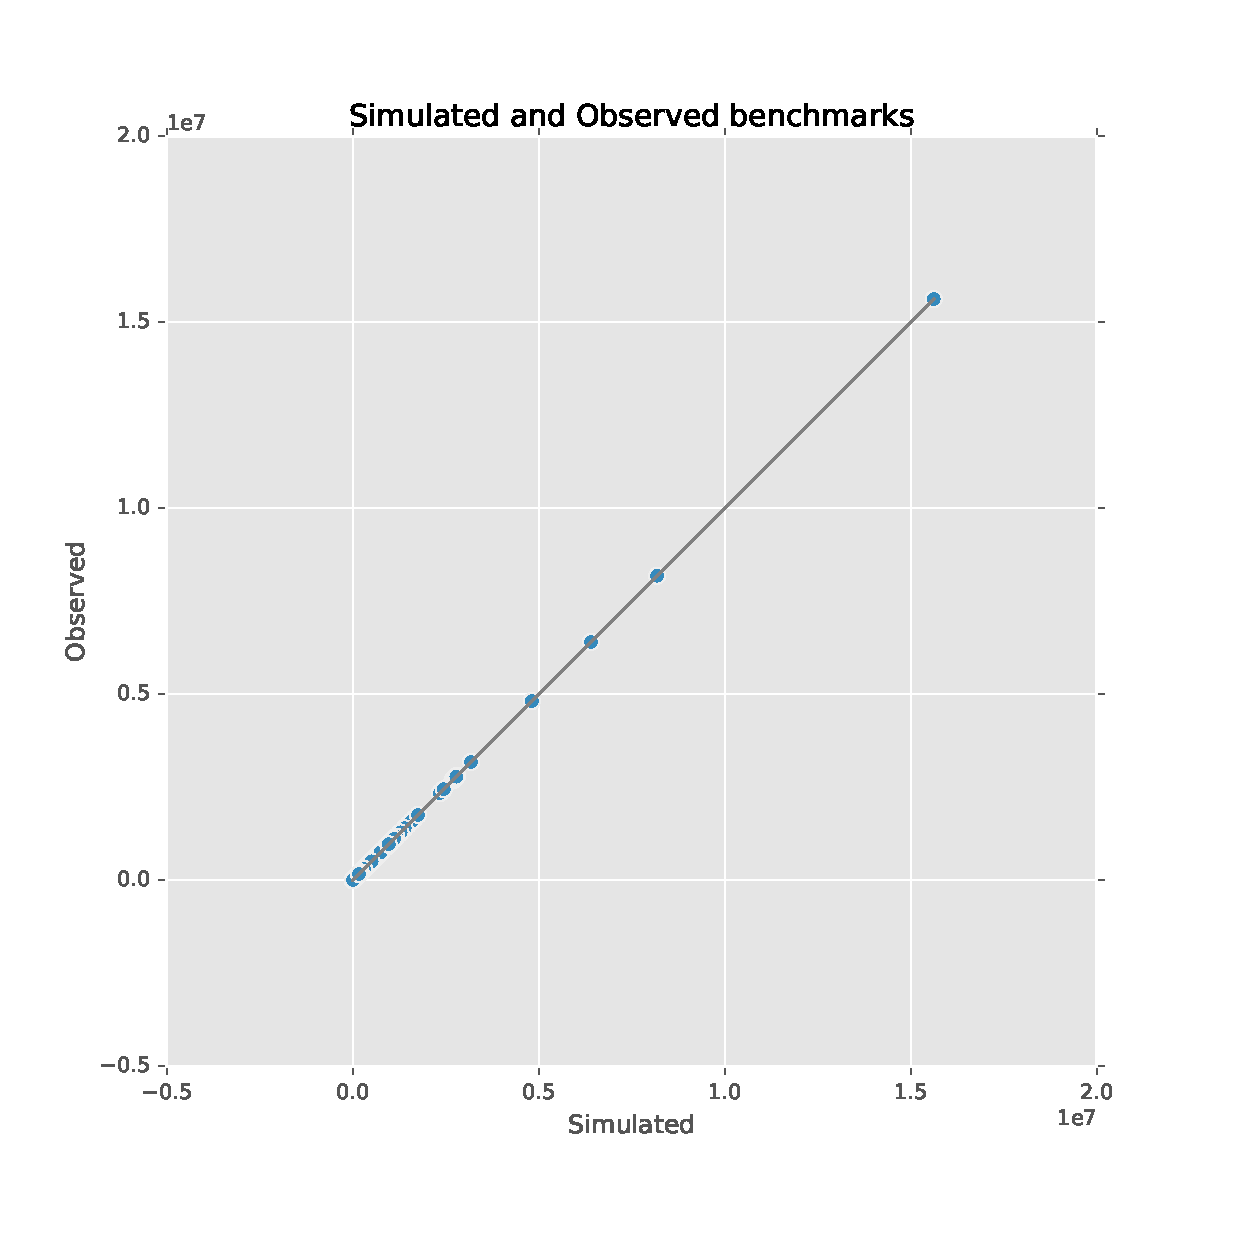
\includegraphics[width=0.9\textwidth]{FIGURES/TAE-scatter}
\caption{Total Absolute Error ($TAE$) of all simulation areas plotted as
simulated vs.\@ observed values}\label{fig:tae}
\end{figure}

The mean $PTAE$ value is 0.9\%. Only 516 areas have a $PTAE$ value higher or
equal to 1\%. If we exclude these 516 areas from the simulation, we achieve a
$PTAE$ value of 0.46\%. Figure~\ref{fig:ptae} shows the $PTAE$ distribution for
all areas with a $PTAE$ value lower that 1\%. We set the 1\% barrier to define
areas on which the re-weighting was effective. This boundary might still be too
high. Setting the $PTAE$ limit at 3\% reduces the number of excluded areas to
10, this would represent 0.09\% of all simulation areas.
\\

\begin{figure}
\centering
\includegraphics[width=0.9\textwidth]{FIGURES/PSAE}
\caption{Error distribution of simulation areas measured as the percentage
total absolute error ($PSAE$)}\label{fig:ptae}
\end{figure}

The performance of the model is very good. This internal validation of the
model only validates the GREGWT re-weighting algorithm. The used library
for the computation of heat demand relies on the German DIN norm which is a
well established method. We still need to keep investigating the process used
for the definition of a synthetic building stock. In this model we have
neglected completely the building geometry, orientation and other energy
relevant attributes.
\\

\subsection{Distribution of Heat Density in Germany}

For the representation of heat demand in space we compute the heat density for
each simulation area as monthly watt-hour per hectare $[Wh/ha \times month]$.
Figure~\ref{fig:mapHeatdensity} shows the heat demand for each month on a
color scale. 
We normalize the color scale for each month. The monthly variation on absolute
heat density cannot be appreciated on this figure because of this
normalization. The aim of the monthly normalization is to identify a variation
on the spatial distribution of heat density  rather than the monthly absolute heat
density.
In terms of heat density we do not observe much change in the pattern through the
year. It is clear that the climate data used as input for the estimation of
heat demand has a strong influence on the result. On the months of July and
August the climate zone 12-Mannheim (see Figure~\ref{fig:climateZones}) is
clearly outlined.
We also appreciate a small decline of heat density during the month of April
in the mid-west part of the country.
The pink spot on the north west part of Germany is the largest urban
agglomeration of the country. The two largest cities can also be spotted on the
map, Hamburg on the north and Berlin on the north-east.
The region surrounding Berlin has a decline on heat density during the month
of July.
\\

\begin{figure}
\centering
\begin{tabular}{lcr}
    January & February & March \\
\includegraphics[width=0.3\textwidth]{FIGURES/heat-January.png}&
\includegraphics[width=0.3\textwidth]{FIGURES/heat-February.png}&
\includegraphics[width=0.3\textwidth]{FIGURES/heat-March.png}\\
    April & May & June \\
\includegraphics[width=0.3\textwidth]{FIGURES/heat-April.png}&
\includegraphics[width=0.3\textwidth]{FIGURES/heat-May.png}&
\includegraphics[width=0.3\textwidth]{FIGURES/heat-June.png}\\
    July & August & September \\
\includegraphics[width=0.3\textwidth]{FIGURES/heat-July.png}&
\includegraphics[width=0.3\textwidth]{FIGURES/heat-August.png}&
\includegraphics[width=0.3\textwidth]{FIGURES/heat-September.png}\\
    October & November & December \\
\includegraphics[width=0.3\textwidth]{FIGURES/heat-October.png}&
\includegraphics[width=0.3\textwidth]{FIGURES/heat-November.png}&
\includegraphics[width=0.3\textwidth]{FIGURES/heat-December.png}\\
\end{tabular}
\caption{Estimated heat density for all the simulated areas through the
year using a color scale normalized for each month}\label{fig:mapHeatdensity}
\end{figure}

The estimated yearly heat demand density for Germany is simply computed as the sum of
the monthly heat densities. Figure~\ref{fig:mapYear} shows the results for the
entire country. On this figure we can clearly identify the large urban
agglomerations in Germany. The important issue to keep in mind is that the
simulation process is occurring at a microlevel. The advantages of this type of
models working at such a low level of aggregation is the ability to simulate
the impact of new national energy policies. A simulation of this type would
allow us to asses and predict the impact of energy relevant policies at the
microlevel. We can identify sections of the population that are particularly
affected by a certain policy and the impact on specific geographical areas.
\\

The presented result show only the developed method for the estimation of heat
demand at a low level of aggregation. The applications of this method for an
energy policy assessment still need to be developed.
\\

\begin{figure}
\centering
\includegraphics[width=0.74\textwidth]{FIGURES/heat-year.png}
\caption{Estimated heat density $[Wh/ha*a]$ for Germany}\label{fig:mapYear}
\end{figure}

We apply this method at a national level because of the data available at this
level. With more data at a lower aggregation level we can apply the exact same
model at a city level. For certain applications the distribution of heat demand
is more attractive at a lower aggregation level. Applications like the planning
of district heat networks need an estimation of heat densities at a lower aggregation level.
Another advantage of a simulation at a city level can be the use of the city
digital cadastre or other datasets describing the building stock at a micro
level. The use of the digital cadastre for the estimation of heat demand allows
us to take further energy relevant parameters of the building stock into
account. See~Mu\~noz~H.\cite{MunozH.2015.MEQ} for a detailed description of the geometry
extraction of a digital cadastre for the simulation of heat demand. The
disadvantage of models based on a digital cadastre is its transferability, many
rural areas of Germany still do not have a digital cadastre. If the aim of this
model is the assessment of national energy policies, we need to take the
entire national building stock into account. Many rural areas might be
particularly affected by a certain policy, not including them because of data
availability would be a systematic error in the model design.
\\

Another advantage of having a completely synthetic building stock-- without a
link to the digital cadastre-- is the ability to project the building stock
into the future under predefined growth scenarios. These type of models can be
used for the assessment of national policies targeting a reduction of carbon
emissions on the building stock. See~Mu\~noz~H.\cite{MunozH.2015.IBPSA.Pop} for an
application of a synthetic building stock projected into the future.
\\

%\begin{figure}
%\centering
%\includegraphics[hight=0.5\linehight]{FIGURES/heat-August_c.png}
%\caption{Estimated heat density $[kWh/ha*month]$ for the month of
%August}\label{fig:mapAug}
%\end{figure}

\section{Conclusions and Further Implementations of Spatial Microsimulation Models for the Analysis of Energy Policy}
\label{sec:conclusions}

The energy policy of a country has always been an essential part of the
national economic planning. Within a policy framework that aims to trigger a
rapid transition towards a low carbon energy infrastructure, we see an
increasingly complex framework that aims to integrate new actors and cope with
new technologies. The complexity attached to the new emerging energy supply systems
needs a better model for the assessment of energy relevant policies at a
national level.
\\

National energy demand models working at an aggregated level are not able to
capture the impact on national policies on individual families. Families of specific
sections of the population might be specially susceptible to a proposed
national policy, we need model able to capture this.
Similar is the case with particular regions in Germany.
Different regions will be affected differently by the proposed policies
implemented at a national or European level.
\\

In this paper we present a robust and quick way to generate a synthetic
population living on a synthetic building stock, enriched with energy relevant
properties, for the entire country. The underlying data generated in this model
can serve as input to all kind of models. The generated data can be used within
an agent based model for the simulation of all type of urban phenomena. Thanks
to the rich survey used in this model we will be able to expand it for the
development of more general urban activity based models. An enrichment of the
survey with time-use data~\cite{MunozH.2014.IBPSA-JP} allows us to represent
not only the building stock, but a detailed description of the occupant activities.
This data can be the base of a transport model working at a micro level or a
detailed model for the estimation of electricity demand based on appliances
use.
\\

Rather than presenting a complete model architecture we updated two open source
R libraries: (1) GREGWT~\cite{MunozH.2015.GREGWTR}, an implementation
of the GREGWT algorithm, used for the re-weighting of the microdata survey; and
(2) HEAT~\cite{MunozH.2015.heat}, an implementation of the German
DIN~18599~\cite{DIN.18599.V}, used for the estimation of heat demand.
The described model is a combination of both libraries.
We aim to develop further small libraries that can be either used individually or
in combination with the above mentioned libraries. We see this development strategy more
sustainable than the development of a complete software architecture.
\\

The challenge ahead is to translate the energy policies in place into machine
readable code in order to establish a basis for the assessment of new energy
policies at a national level.
\\

\bibliographystyle{plain}
\bibliography{ABMUS_munozh.bib}

\end{document}
